% Satellite Missions
In order to better observe freshwater resources, recent satellite missions have provided massive amounts of data, such as precipitation from the Tropical Rainfall Measurement Mission (TRMM) and the Global Precipitation Measurement (GPM) mission, surface soil moisture from the Soil Moisture Active and Passive (SMAP) mission, total water storage change from the Gravity Recovery and Climate Experiment (GRACE) and the GRACE Follow-on (GRACE-FO) mission. In particular, surface deformation data derived from interferometric synthetic aperture radar (InSAR) (1992-present) can be used for characterizing groundwater levels and storage properties in confined aquifers, the critical metric needed for effective groundwater management. While spaceborne Earth-observing missions have provided large amounts of data that can be used to study freshwater resources, these data have been greatly under-utilized in operational water management practices. A grand challenge we need to address today is how to assimilate satellite and in-situ data into quantitative, predictive and computational groundwater models to better assist decision making.

The Rio Grande Decision Support System (RGDSS) is a MODFLOW model of the SLV that is used to predict head levels in the confined aquifer  .  Head data over the active area of water use are sparse in 1978, but grow more robust to the present although the monitoring data points are unequally distributed . The lack of historical and well-distributed head data impacts the accuracy of the modeling.  There is great interest in the ability to assimilate satellite and in-situ data into quantitative, predictive and computational groundwater flow models to better assist decision making.

Currently, the Rio Grand Decision Support System (RGDSS), which includes a hydrogeologic database and a MODFLOW finite-difference groundwater flow model, 

The conceptual RGDSS hydrogeologic model of the SLV consists of five distinct hydrogeologic layers \citep{RGDSS}. 


\subsubsection{Water Balance Model}
Understanding the availability of freshwater resources requires measurement of key components in the freshwater cycle shown in Figure \ref{fig:watercycle}. Here we consider the surface water and boundary layer as a single element, denoted surface water. The net freshwater fluxes can be approximated by the following equation:
\begin{align}
\Delta SM +\Delta S^s +\Delta S^u + \Delta S^c = P-ET-Q
\label{eq:waterBalance}  
\end{align}
where $P$ is precipitation, $ET$ is evapotranspiration, $Q$ is the river runoff. $\Delta SM$ is the change in soil moisture, $\Delta S^s$ is the change in surface water storage in rivers and lakes, $\Delta S^u$ is the change in unconfined aquifer storage, and $\Delta S^c$  is the change in confined aquifer storage.

\begin{figure}
\noindent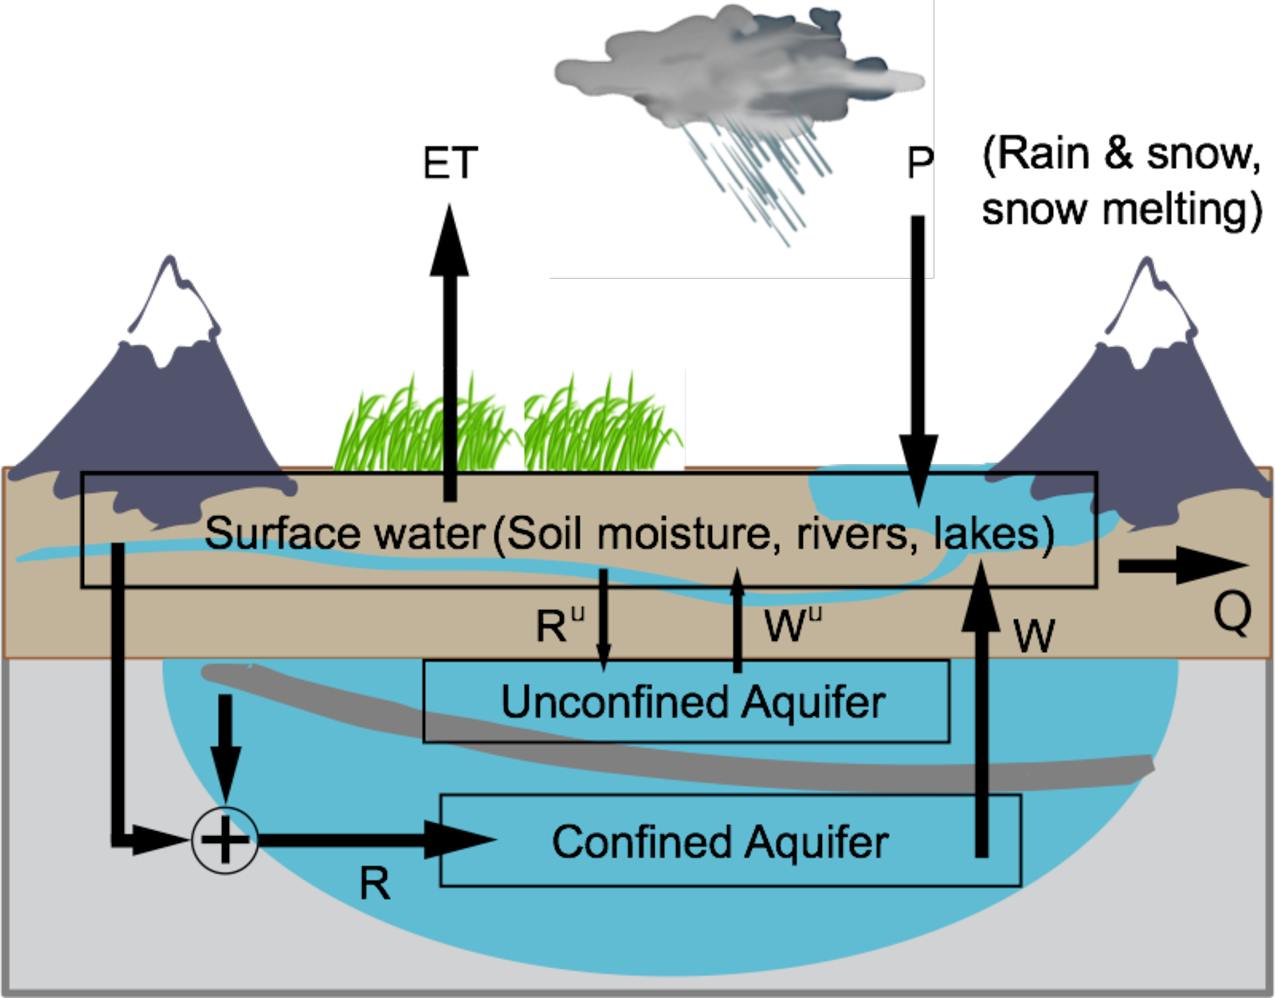
\includegraphics[width=0.6\textwidth]{Figures/watercycle.pdf}
\caption{Water balance model. In this model surface water and soil moisture are combined into the “surface water” box.  The terms marked in blue are the key elements of the water balance equation; their interrelationships are discussed in Equation \ref{eq:waterBalance}.}
\label{fig:watercycle}
\end{figure}

The change in confined aquifer storage $\Delta S^c$ can be further expressed as:
\begin{align}
\Delta S^c = R - W
\label{eq:confinedStorage}  
\end{align}
where $W$ is the withdrawal from the confined aquifer and R is the recharge. Given a \textcolor{red}{minimum safe storage level for the confined aquifer} $\Delta S^{C-min}$, we can manage the storage of the confined aquifer by scheduling withdrawals such that withdrawal ceases when (in our convention withdrawal leads to negative $\Delta S^c$):
\begin{align}
\Delta S^c = P-ET-Q-\Delta SM - \Delta S^s - \Delta S^u = R-W < \Delta S^{C-min}
\label{eq:safelimit}  
\end{align}
Note that $\Delta S^c$  can be considered as a source term describing the forcing of water into the confined aquifer.  We therefore introduce an additional notation to emphasize its role as a source and its explicit dependence on both space and time:
\begin{align}
U(x;t) = \Delta S^c
\label{eq:force}  
\end{align}

\begin{figure}
\noindent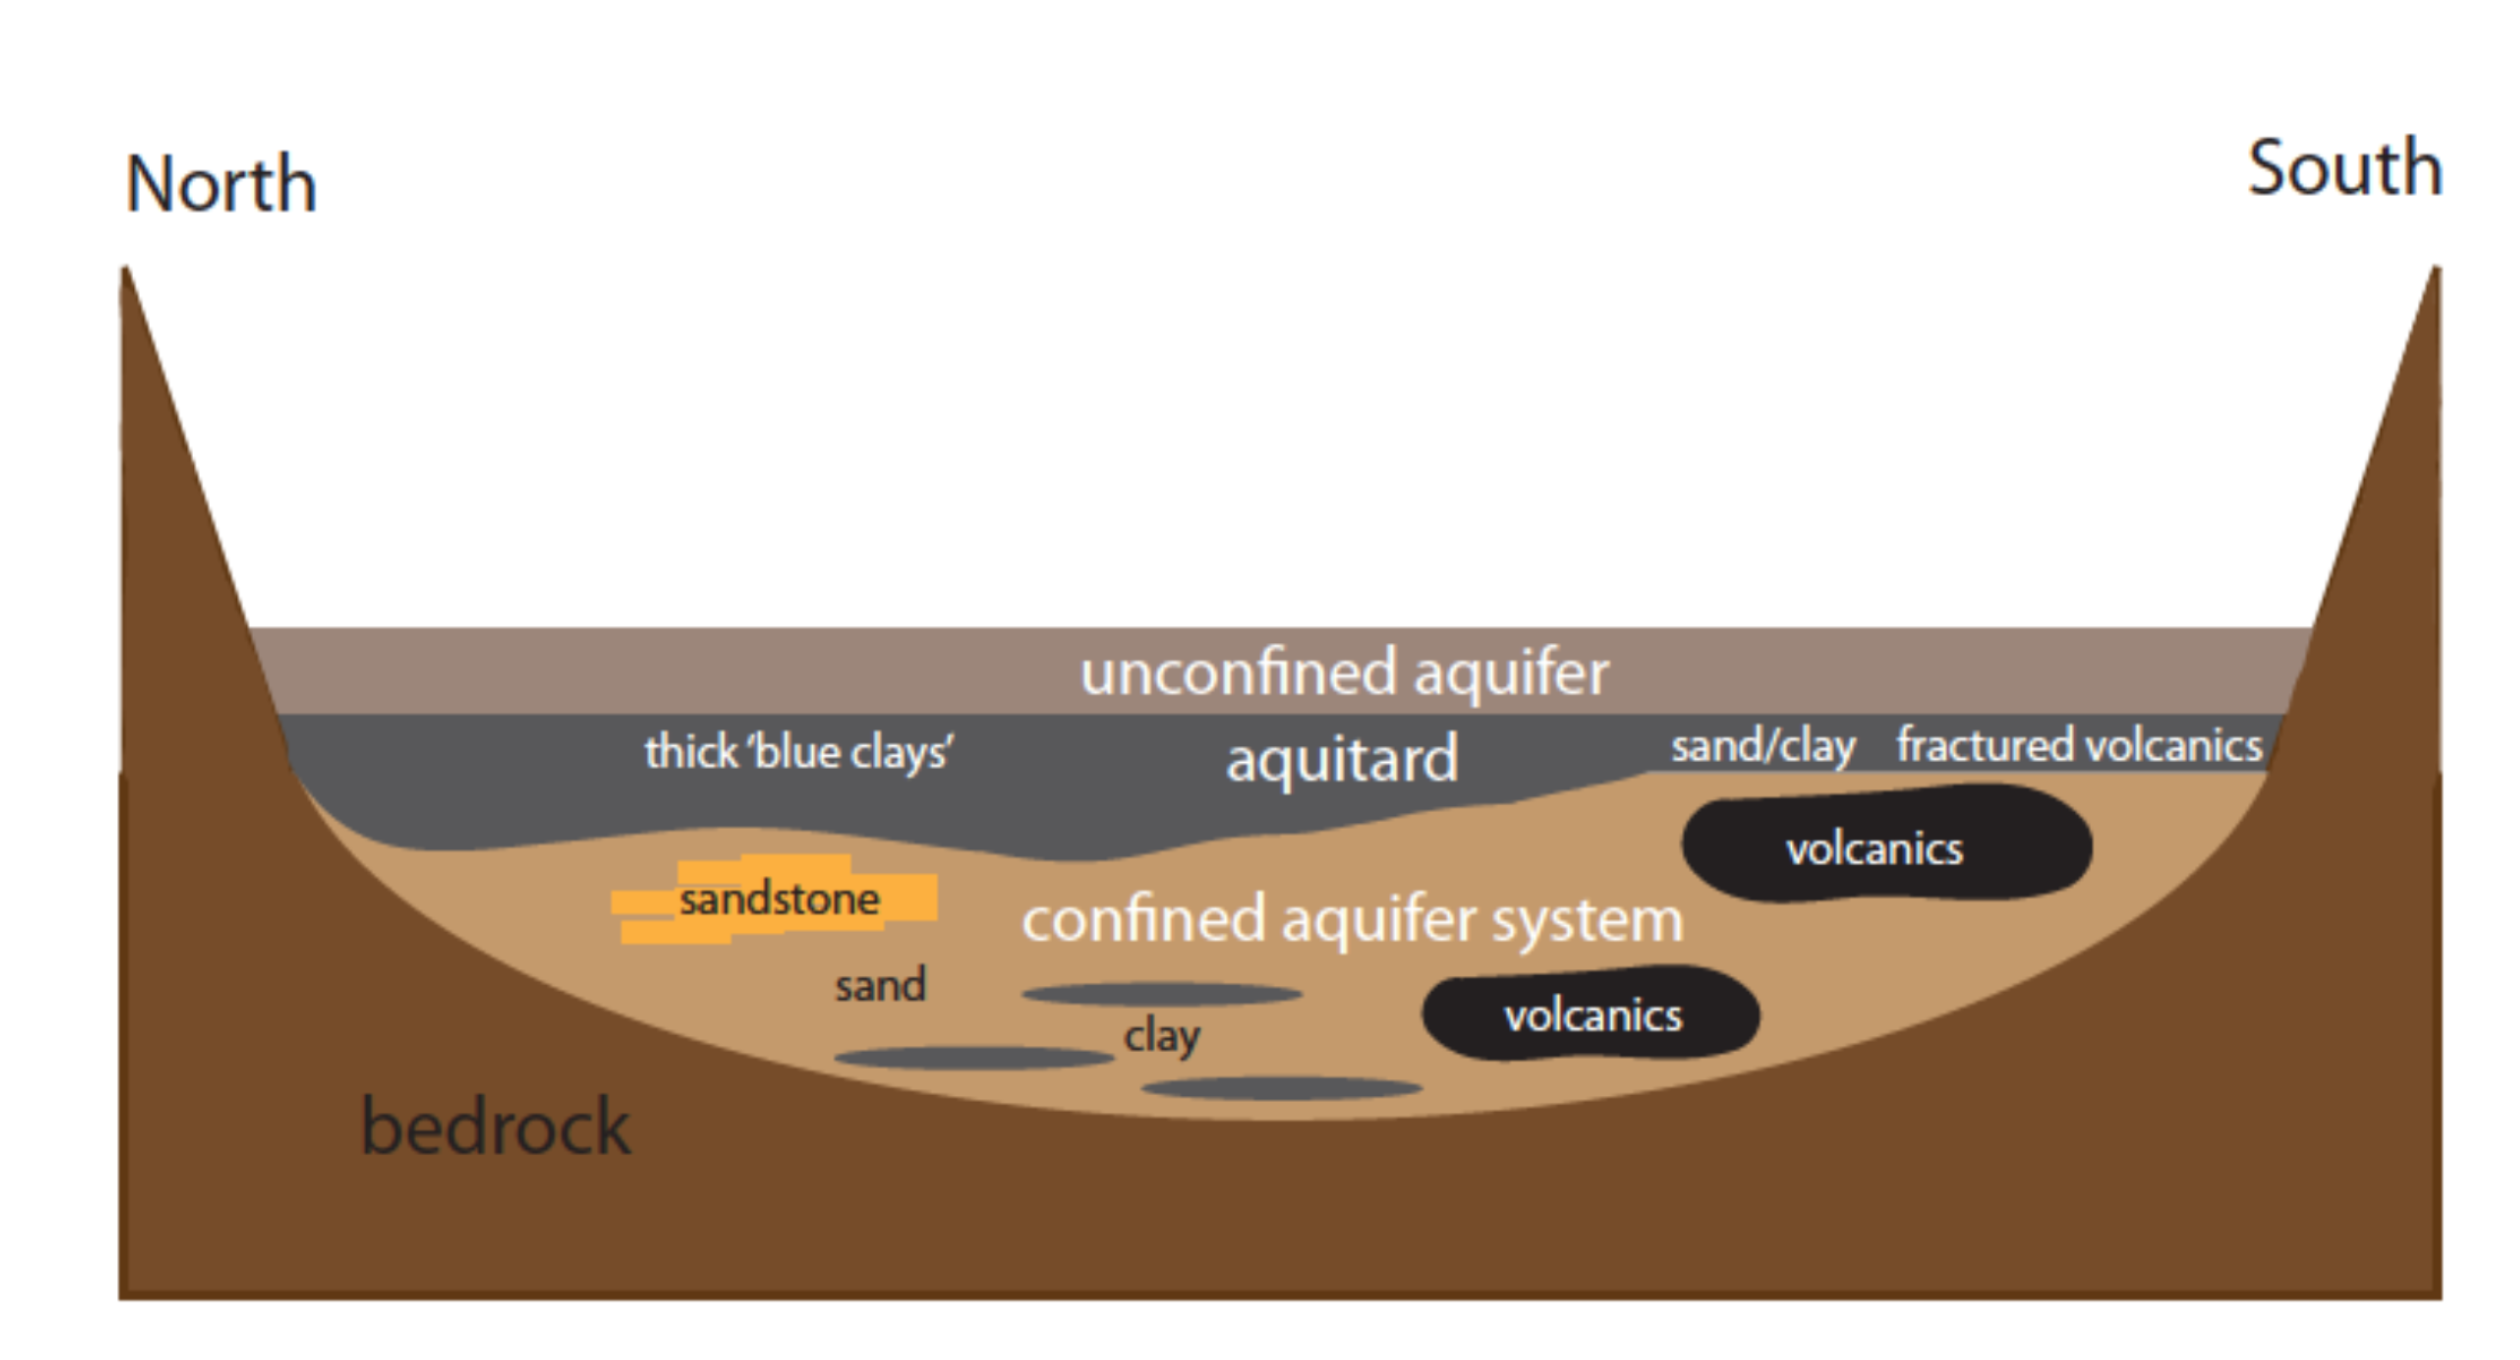
\includegraphics[width=0.9\textwidth]{Figures/SLVaquifers.png}
\caption{A schematic showing the variable geology of the hydrogeologic layers from north to south in the San Luis Valley (J. Reeeves, 2013).}
\label{fig:slv-aquifers}
\end{figure}